% -*- mode:flyspell; mode:latex  -*-

%%% Local Variables:
%%% TeX-master: "mu2e-36575"
%%% End:

%%%%%%%%%%%%%%%%%%%%%%%%%%%%%%%%%%%%%%%%%%%%%%%%%%%%%%%%%%%%%%%%%%%%%%%%%%%%% 
\section{Track quality selections}

%%%%%%%%%%%%%%%%%%%%%%%%%%%%%%%%%%%%%%%%%%%%%%%%%%%%%%%%%%%%%%%%%%%%%%%%%%%%%%
\subsection{\MuToEm\  channel}
\label{sec:mumem_channel}

Selection of correctly reconstructed tracks plays a critical role in the search, and 
to improve rejection of poorly reconstructed  tracks, an MVA-based technique is used.
A MLP ANN is trained to distinguish between correctly reconstructed tracks and mis-reconstructed
ones; good tracks are selected by requiring the ANN score to be above a certain value.

In the base version of the Mu2e Offline (v9\_0\_5) a track quality ANN has been trained only for PAR tracks,
we performed a similar training for the DAR tracks.
%
Following \cite{MU2E_4595_ANN_TRAINING}, we used the ROOT TMVA package to train an 
MLP ANN with 8 input variables and one hidden layer. The following eight variables
were used as inputs:

\begin{itemize}
\item
  {\bf na } : the number of active hits remaining on the track 
  after the Kalman fit and used in the calculation of the fit $\chi^2$
\item
  {\bf nafract} : the ratio of the number of active hits to the total number
  of hits (number of hits after the seed fit)
\item
  ${\bf log_{10}(fcons)}$ : {\bf fcons}, or the fit consistency, 
  is a probability-minded derivative of the track fit $\chi^2$. The logarithm
  of it is taken for numerical considerations
\item
  {\bf momerr} : the uncertainty on the reconstructed track momentum, returned by the fitter
\item
  {\bf t0err} : the uncertainty on the reconstructed track time, $T_0$, returned by the fitter
\item
  {\bf fda} : the fraction of doublet active hits over total number of active hits
\item
  {\bf fza } : the fraction of active hits with undefined drift direction
\item
  {\bf fma } : the fraction of straws with hits over the number of straws geometrically crossed by the track
\end{itemize}

The ANN training is aimed to optimize the separation of electron tracks reconstructed correctly, 
defined as $ |\Delta{P}| = |P_{reco}-P_{true}| < 0.25$ MeV/c, or approximately within $2\sigma$ of
the true value, from tracks with significantly larger reconstructed momentum, defined as
$\Delta{P} > 0.7$ MeV/c, or approximately $5\sigma$ above the true value.
%
Comparison between $P_{true}$ and $P_{reco}$ was performed in a plane corresponding to the tracker front.
%
Tracks with |D0| < 100 mm and 0.5 < \tandip < 1 were used to train the ANN.

To choose between the PAR-based and DAR-based fitters, we compared performance of the
trained DAR ANN to the performance of the default for the Mu2e Offline v9\_0\_5 PAR ANN.
%
We compared the performance of the two methods using the CD3 choice for the signal region:
103.85 < P < 104.90 MeV/c and $T_0 > 700$ ns.
%
Figure \ref{fig:mumem_ann_operational_point_choice} shows the expected DIO background plotted
versus the CE reconstruction efficiency. Both are plotted in relative units, normalized
to the DIO background and CE efficiency of the PAR track selection with the default
cut on the ANN score $S_{PAR} > 0.8$.
%
Square markers represent the PAR track selection and circle markers represent the DAR track selection;
red and black colors correspond to the conversion electron signal MC with 1 and 2 batch mode pileup 
datasets respectively.
%
In all cases the background model comes from the DIO-weighted fele2s51b1 dataset - 
flat energy electron MC with 1 batch mode pileup. 

As follows from Figure \ref{fig:mumem_ann_operational_point_choice},
using the DAR tracks increases the signal acceptance by 4-5\% with respect to PAR tracks for the same expected
background level. One can also see, that the Mu2e Offline default choice of the PAR ANN operational point
is quite close to the optimum - after the (1,1) point the PAR background starts increasing much faster than
the PAR signal, and the increase by 5\% comes along with a x2 higher DIO background.

For the DAR tracks, improving the signal acceptance by the same 5\% with respect to the default
Offline selection does not cost extra background. This determines the choices for the SU2020 analyses: 

\begin{itemize}
\item
  SU2020 analyses use DAR tracks
\item
  the ANN operational point corresponds to the cut on the output of $S_{DAR} > 0.2$.
\end{itemize}

\begin{figure}[H]
\begin{tikzpicture}
  \node[anchor=south west,inner sep=0] at (0,0.) {
    % \node[shift={(0 cm,0.cm)},inner sep=0,rotate={90}] at (0,0) {}
    \makebox[\textwidth][c] {
      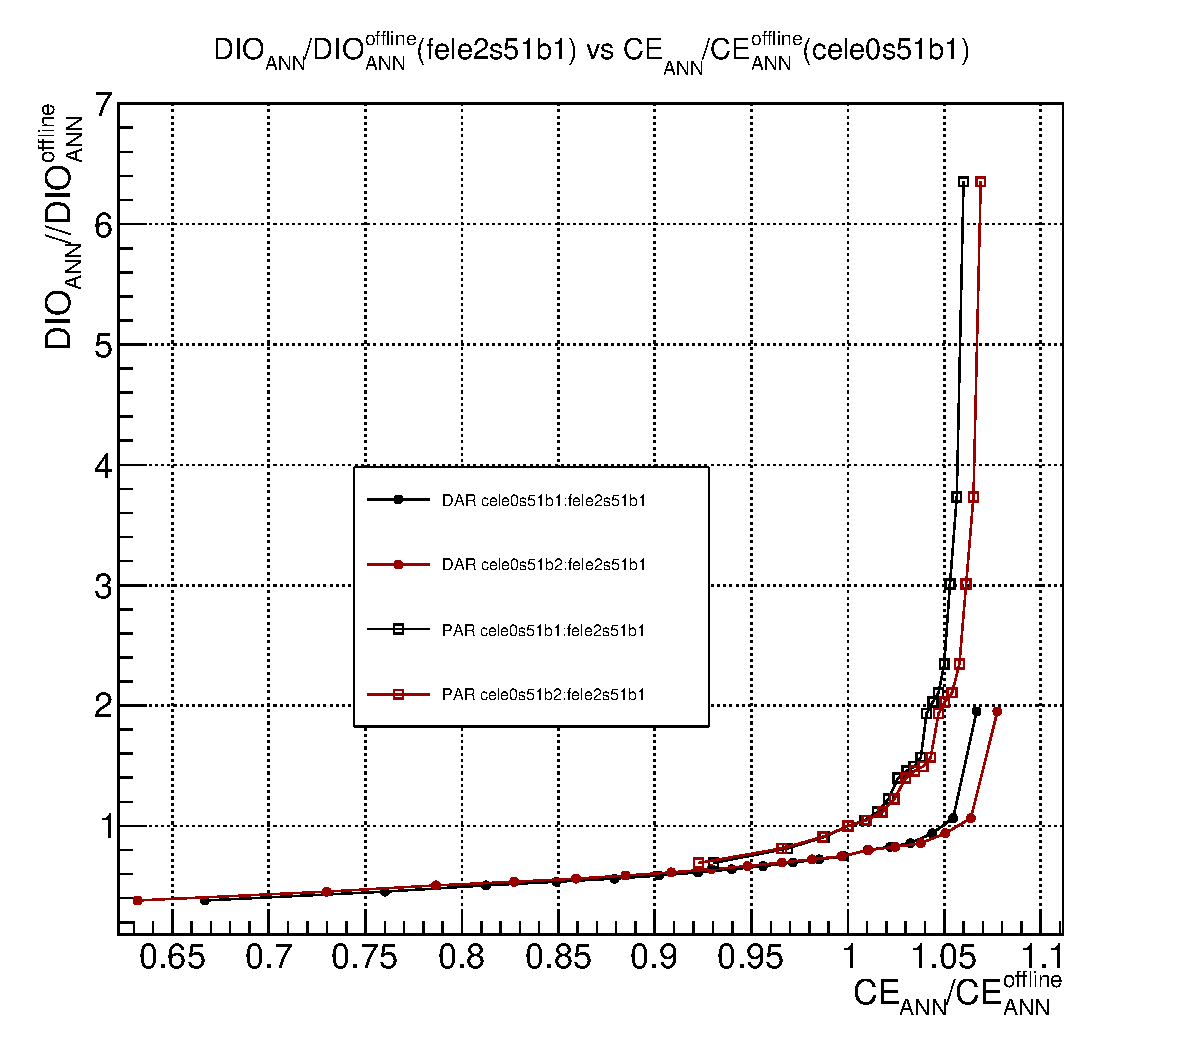
\includegraphics[width=0.8\textwidth]{figures/pdf/mumem_trq_ann_signal_vs_background}
    }
  };
  % \node [text width=6cm, scale=0.8] at (4.5,6.4) {mu2e-18894 by Kevin Lynch and Jim Popp};
\end{tikzpicture}
% \captionof{figure} {
\caption{
  \label{fig:mumem_ann_operational_point_choice}
%  \strike{Choice of the ANN operational point.}
  Relative DIO background versus relative signal acceptance.
  The expected DIO background, relative to the DIO background corresponding to the default Offline
  PAR ANN track selection,
  is plotted versus efficiency of the conversion electron signal acceptance, normalized to the efficiency
  of the signal selection using the default Offline PAR ANN.
  PAR curves, by construction, go through the point (1,1) which corresponds to default Offline PAR track selection
  of $S_{PAR} > 0.8$.
  Background : DIO-weighted {\bf fele2s51b1}, signal: {\bf cele0s51b1} (red), or {\bf cele0s61b2} (black).
}
\end{figure}

Figure \ref{fig:mumem_dar_vs_par_ann} compares the track momentum resolution distributions 
for DAR and PAR tracks reconstructed in the conversion electron plus two batch mode pile-up dataset,
{\bf cele0s61b2}, using either a fixed background or a fixed signal efficiency operational point. 
In Figure \ref{fig:mumem_dar_vs_par_ann}(a), the operational points for the DAR
and PAR track selections are chosen to give the same expected background -
in Figure \ref{fig:mumem_dar_vs_par_ann}(b), the same track selection efficiency. A higher 
high-momentum tail in the distribution for PAR tracks is clearly visible in both operational points.

\begin{figure}
\hspace{-0.6in}
\begin{tikzpicture}
  \node[anchor=south west,inner sep=0] at (0,0.) {
    % \node[shift={(0 cm,0.cm)},inner sep=0,rotate={90}] at (0,0) {}
    % \makebox[\textwidth][c] {
    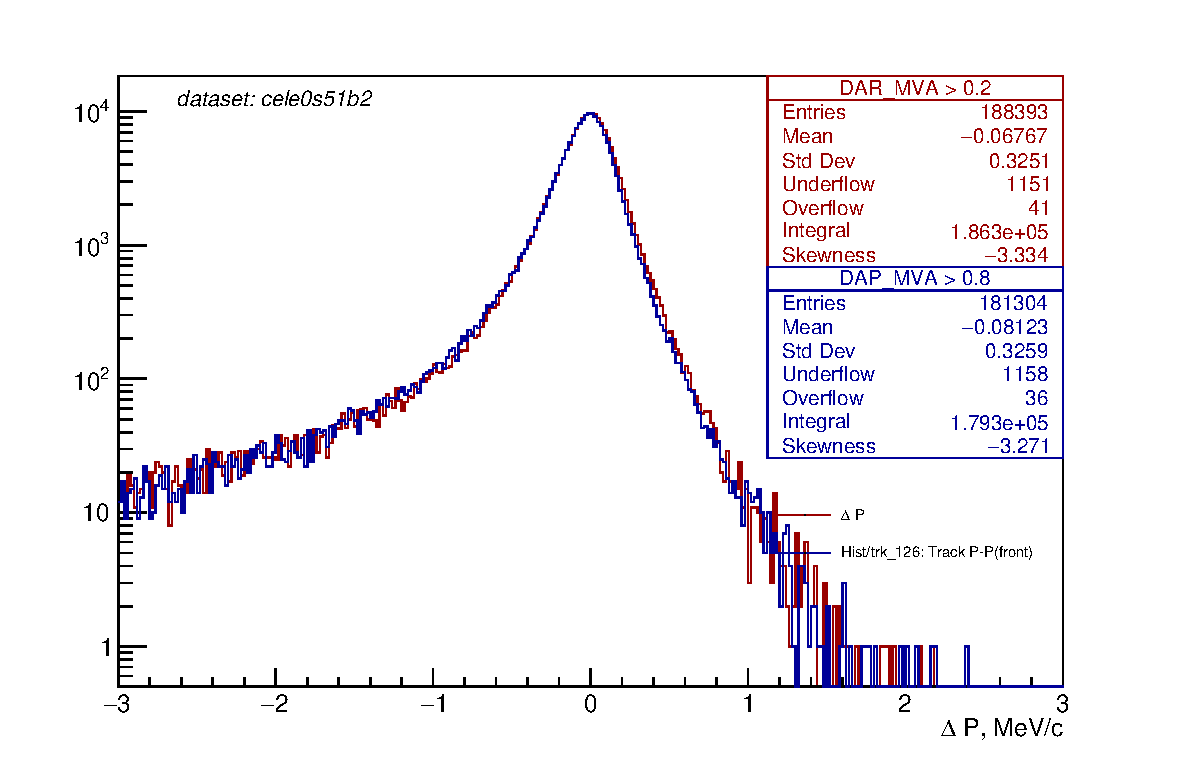
\includegraphics[width=0.64\textwidth]{figures/pdf/figure_00114_cele0s51b2_track_comp_ffff_1070_trk_214_vs_126_dpf}
    % }
  };
  \node [text width=1cm, scale=0.8] at (3.,4.5) {(a)};
  \node[anchor=south west,inner sep=0] at (10.5,0.) {
    % \node[shift={(0 cm,0.cm)},inner sep=0,rotate={90}] at (0,0) {}
    % \makebox[\textwidth][c] {
    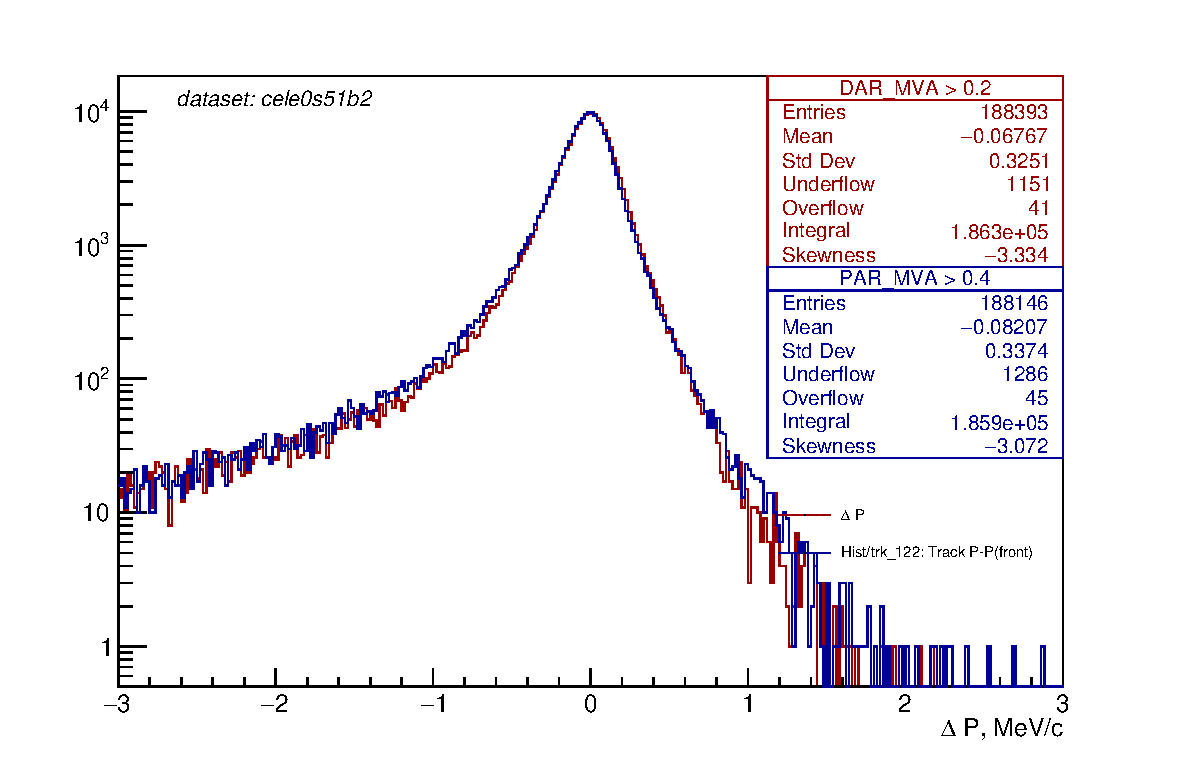
\includegraphics[width=0.64\textwidth]{figures/pdf/figure_00116_cele0s51b2_track_comp_ffff_1070_trk_214_vs_122_dpf}
    % }
  };
  \node [text width=1cm, scale=0.8] at (13.5,4.5) {(b)};
\end{tikzpicture}
% \captionof{figure} {
\caption{
  \label{fig:mumem_dar_vs_par_ann}
  DAR vs PAR track selection efficiency for two operational points: 
  (a): DAR ($S_{DAR} > 0.2$) and PAR ($S_{PAR} > 0.8$) selections correspond to the same background level ;  
  (b): DAR ($S_{DAR} > 0.2$) and PAR ($S_{PAR} > 0.4$) track selections correspond to the same efficiency
  The right-side tail, the most severely mis-reconstructed tracks, is a measure of the track selection
  quality.
}
\end{figure}

Improvements in the track reconstruction, for the same selection efficiency, result in significantly improved
rejection of mis-reconstructed tracks. Figure \ref{fig:dio_delta_p_1036_1050} shows the $\Delta{P}$ distribution
for the simulated DIO electrons (DIO-weighted {\bf fele2s51b1}) with reconstructed track momentum in [103.6, 105.0] MeV/c.
From that distribution one can easily see the importance of the relative contribution
of tracks with $\Delta{P}$ above a certain threshold. In particular, tracks with significantly mis-reconstructed
momentum, $\Delta{P} > 0.5$ MeV, represent about 0.23 of the expected DIO background (which is about 50\% lower
than the previous estimate of 0.355 for the same momentum window in \cite{MU2E_4595_ANN_TRAINING}).

\begin{figure}
  \begin{tikzpicture}
    \node[anchor=south west,inner sep=0] at (0,0.) {
      % \node[shift={(0 cm,0.cm)},inner sep=0,rotate={90}] at (0,0) {}
      \makebox[\textwidth][c] {
        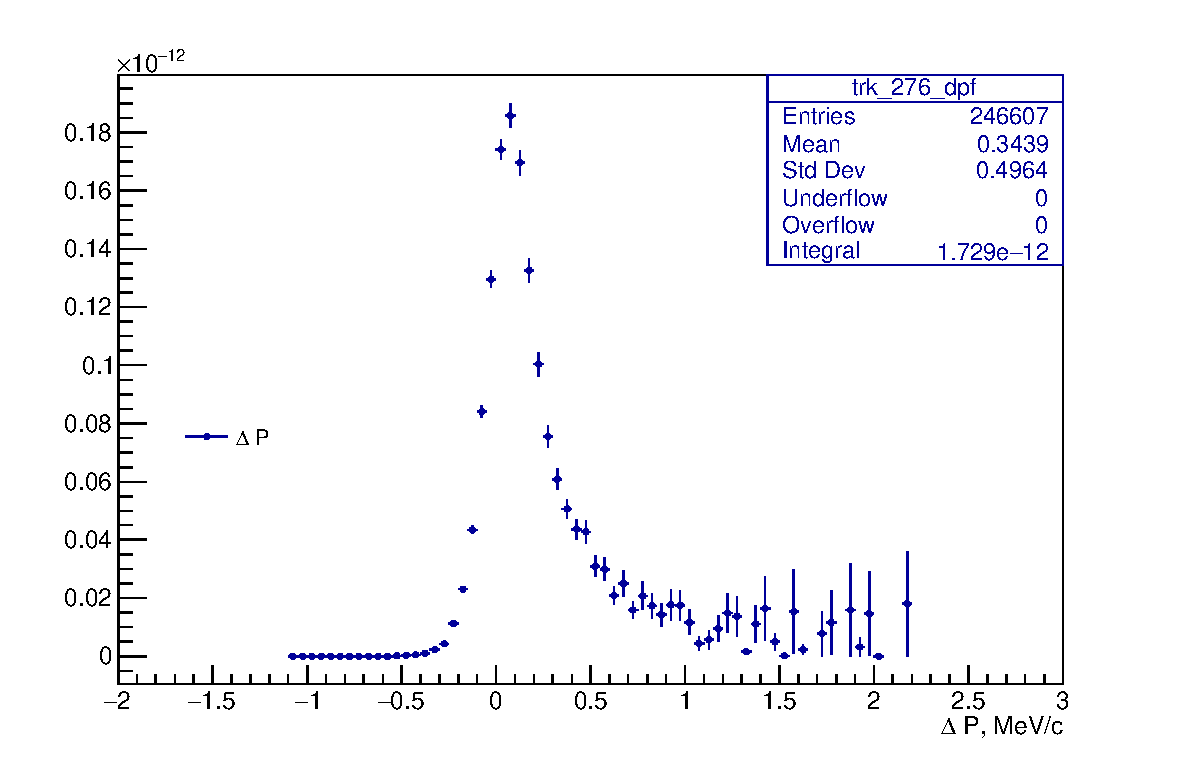
\includegraphics[width=0.99\textwidth]{figures/pdf/figure_00111_fele2s51b1_track_comp_ffff_1070_trk_276_dpf}
      }
    };
    % \node [text width=6cm, scale=0.8] at (4.5,6.4) {mu2e-18894 by Kevin Lynch and Jim Popp};
  \end{tikzpicture}
  % \captionof{figure} {
  \caption{
    \label{fig:dio_delta_p_1036_1050} 
    $\Delta P ~=~ P_{reco} -P_{true}$ distribution for the simulated DIO background in the region [103.6,105.0] MeV.
    77.2\% of the reconstructed events in this region are expected to have $\Delta P < 0.5$ MeV/c
  }
\end{figure}

As a cross-check, we used the TMVA package to train a BDT-based track quality classifier.
Similar to \cite{MU2E_33150_ANN_TRAINING}, we found that the MLP ANN performed slightly better,
so the current analysis uses a MLP ANN-based track quality selection. 
To explore the parameter space, the definition of a ``mis-reconstructed track'' has been varied
and a similar ANN has been trained to discriminate tracks reconstructed with $|\Delta{P}| < 0.25$ MeV/c 
from tracks with $\Delta{P} > 0.6$ MeV/c.
No improvement in the DIO suppression in the region [103.85, 104.9] MeV/c was observed. 

%%%%%%%%%%%%%%%%%%%%%%%%%%%%%%%%%%%%%%%%%%%%%%%%%%%%%%%%%%%%%%%%%%%%%%%%%%%%%%
\newpage
\subsection{\MuToEp\ channel}
\label{sec:mumep_channel}

To select tracks in the \MuToEp\ channel, a conversion positron MC with one-batch mode pileup dataset
({\bf cpos0s51b1}) has been used to train an MLP ANN to discriminate between well reconstructed and
mis-reconstructed positron tracks.
%
The ANN configuration and the definitions of well reconstructed and mis-reconstructed tracks are
the same as described in Section \ref{sec:mumem_channel}.

Figure \ref{fig:mumep_trq_ann} compares the expected background vs the signal efficiency curves,
relative to the default Offline positron selection (as in Figure \ref{fig:mumem_ann_operational_point_choice}),
for PAR (squares) and DAR  (circles) tracks. The background definition, however, is different.
Unlike in \MuToEm\ channel, in \MuToEp\ channel there is no well defined background process whose contribution
could be used as a measure of mis-reconstruction. 
The RMC contribution depends on the assumptions about the RMC photon momentum distribution and,
in particular, its endpoint. Because of this, the background in Figure \ref{fig:mumep_trq_ann} 
is defined as the expected number of events with mis-reconstructed momentum $\Delta{P} > 1.0$ MeV.
%
The signal is integrated over the [90.5,92.5] MeV/c momentum window.

Figure \ref{fig:mumep_trq_ann}.(b) shows the same performance curves as Figure \ref{fig:mumep_trq_ann}.(a),
but with the vertical axis in logarithmic scale. It is interesting to see that for a given background
definition, the background increases exponentially with the signal acceptance for both types of tracks.
For the same signal acceptance, the ANN-based selection of DAR tracks results in lower
backgrounds, so the sensitivity estimate in the \MuToEp\ channel also uses the DAR tracks.

For the choice of the operational point, the cut $S_{DAR} > 0.2$ improves the signal acceptance
by 10\%, while increasing the background by 15\%. Relaxing the cut and moving the cut value to $S_{DAR} > 0.15$
adds another 2\% to the CP acceptance, while the background grows much faster and
becomes $B_{DAR}/B_{PAR}^{default} = 1.5,$ Thus, the default cut on $S_{DAR}^+$ is the same as
in the electron channel:  $S_{DAR}^+ > 0.2$

An attempt to train a similar ANN for PAR tracks didn't result in an improvement of an ANN-based track
selection. As the training parameters in both cases are essentially the same, this result is somewhat 
surprising and may be pointing to a potential of further improvements. 

\begin{figure}[H]
  \hspace{-0.6in}
  \begin{tikzpicture}
    \node[anchor=south west,inner sep=0] at (0,0.) {
      % \node[shift={(0 cm,0.cm)},inner sep=0,rotate={90}] at (0,0) {}
      % \makebox[\textwidth][c] {
      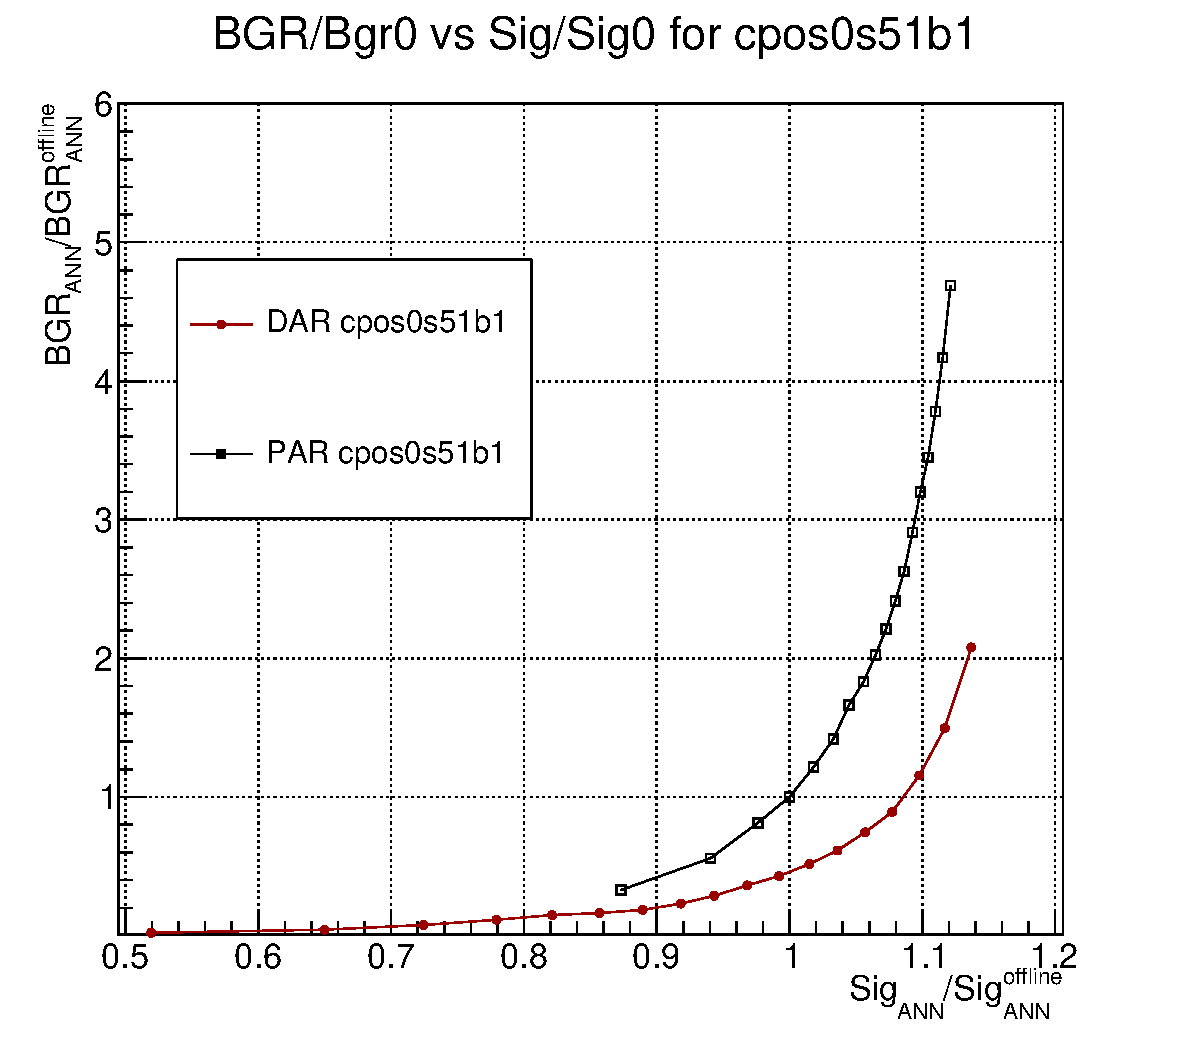
\includegraphics[width=0.55\textwidth]{figures/pdf/mumep_trq_ann_signal_vs_background_lin}
      % }
    };
    \node [text width=1cm, scale=1.0] at (3.,3.5) {(a)};
    \node[anchor=south west,inner sep=0] at (10,0.) {
      % \node[shift={(0 cm,0.cm)},inner sep=0,rotate={90}] at (0,0) {}
      % \makebox[\textwidth][c] {
      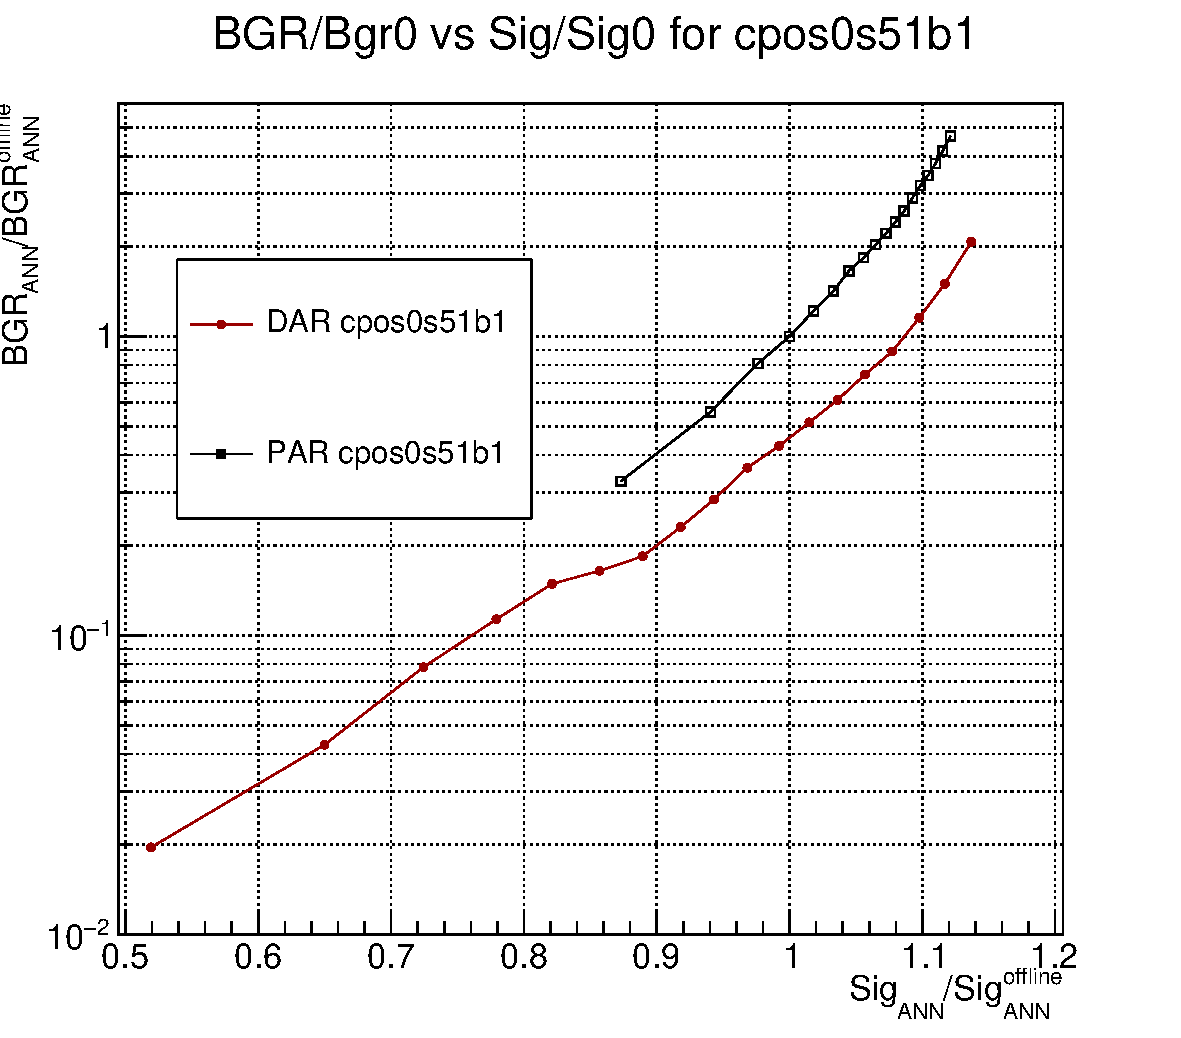
\includegraphics[width=0.55\textwidth]{figures/pdf/mumep_trq_ann_signal_vs_background_log}
      % }
    };
    \node [text width=1cm, scale=1.0] at (13.,3.5) {(b)};
  \end{tikzpicture}
  % \captionof{figure} {
  \caption{
    \label{fig:mumep_trq_ann} 
    DAR (Circles) vs PAR (squares) background vs signal window efficiency.
    Signal: {\bf cpos0s51b1}, 90.5 < P < 92.5 MeV/c ;
    background:{\bf cpos0s51b1} , tracks with $\Delta{P} > 1.0$ MeV.
    Both signal and background are measured in units of signal and background efficiency
    corresponding to the selection using the default Offline v9\_0\_5 ANN-based track
    selection, $S_{PAR}^+ > 0.8$.
  }
\end{figure}

%%%%%%%%%%%%%%%%%%%%%%%%%%%%%%%%%%%%%%%%%%%%%%%%%%%%%%%%%%%%%%%%%%%%%%%%%%%%%%
\subsection{Testing charge symmetry of the ANN-based track selection}

It is worth noting that the track parameters used for ANN training do not depend explicitly
on the reconstructed track sign. One could therefore expect the efficiency of the ANN-based
track selection to be charge-symmetric. To check this hypothesis, Figure \ref{fig:su2020_mva_test_dar}
compares the efficiency of the electron trained ANN-based selection for 105 MeV electrons and 105 MeV positrons.

Figure \ref{fig:su2020_mva_test_dar} confirms that for the same track momentum, the ANN-based selection
is charge-symmetric with an accuracy better than 0.5\%. The third, and the only visible, distribution
in Figure \ref{fig:su2020_mva_test_dar} corresponds to 105 MeV electron tracks selected
using the ANN trained on 92 MeV positrons as described in Section \ref{sec:mumep_channel}. One would expect
the efficiency of this selection to be sub-optimal, but rather surprisingly, the efficiency is reduced by
less than 4\%.
Observed charge symmetry allows to use one common ANN, trained using 105 MeV/c tracks, for track selection
in all \MuToEm\ search analyses and another common ANN, trained using 92 MeV/c tracks, for track selection 
in all \MuToEp\ search analyses.

\begin{figure}
  % \hspace{-0.6in}
  \begin{tikzpicture}
    \node[anchor=south west,inner sep=0] at (0,0.) {
      % \node[shift={(0 cm,0.cm)},inner sep=0,rotate={90}] at (0,0) {}
      \makebox[\textwidth][c] {
        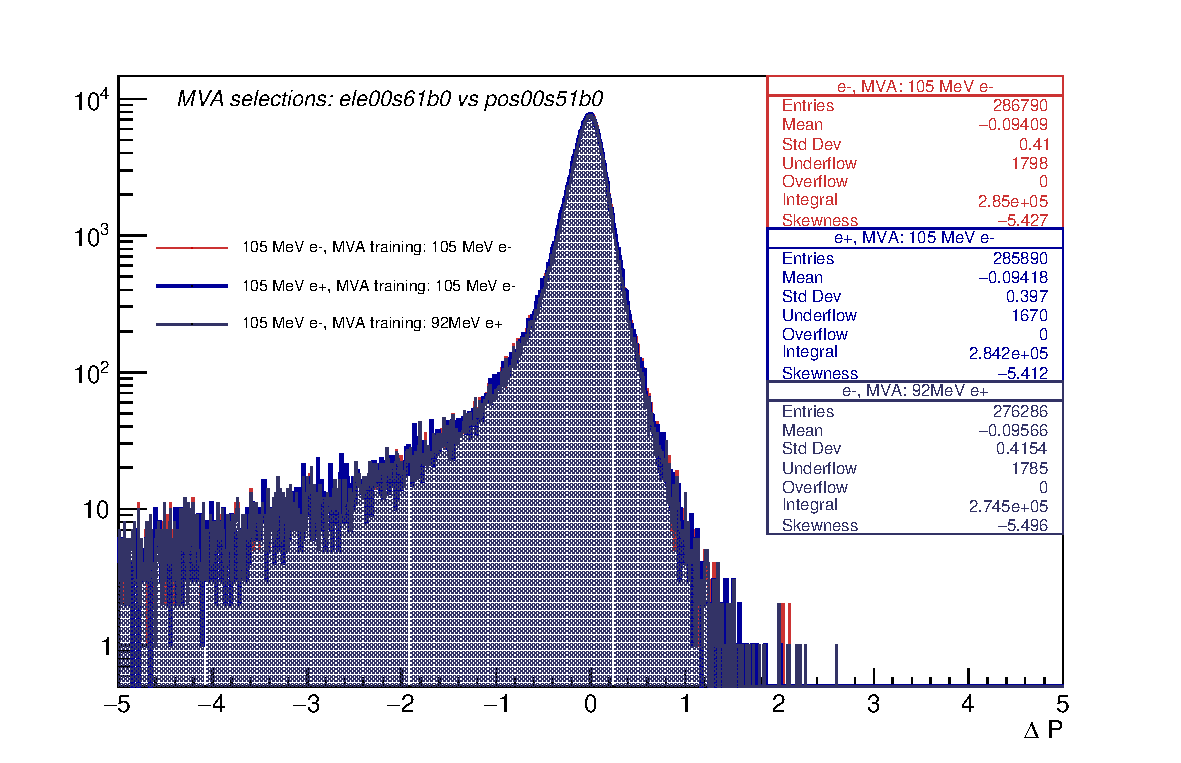
\includegraphics[width=0.95\textwidth]{figures/pdf/figure_00231_su2020_mva_test_dar}
      }
    };
    % \node [text width=6cm, scale=0.8] at (4.5,6.4) {mu2e-18894 by Kevin Lynch and Jim Popp};
  \end{tikzpicture}
  % \captionof{figure} {
  \caption{
    \label{fig:su2020_mva_test_dar} 
    105 MeV/c electrons and positrons selected using an ANN trained on 105 MeV/c electrons,
    and 105 MeV/c electrons selected using an ANN trained on 92 MeV/c positrons
  }
\end{figure}


%%%%%%%%%%%%%%%%%%%%%%%%%%%%%%%%%%%%%%%%%%%%%%%%%%%%%%%%%%%%%%%%%%%%%%%%%%%%%%
\subsection{Track selection cuts summary}
\label{sec:track-selection_cuts_summary}
  
For SU2020 analyses, a well reconstructed track is a DAR track satisfying the following requirements:

\begin{itemize}
\item
  the track impact parameter, ${\bf d_0}$, is consistent with the track coming from the stopping target: 
  ${\bf |d_0|} < 100$ mm. We note that ${\bf d_0}$ is calculated at a point of closest approach of
  the reconstructed trajectory to the beam axis, which is located inside the Mu2e tracker and 
  % {\blue which point inside the tracker?} - point of the trajectory closest approach to the beam axis
  several meters away from the stopping target,
  and therefore cannot be directly compared with the radius of the stopping target foils ;
\item 
  the track dip angle, $\lambda = 90^o - \alpha$, where $\alpha$ is the track angle with respect 
  to the solenoid axis, is within $ 0.5 < \tan{\lambda} < 1$. 
  The choice of the lower cutoff value, 0.5, is not currently dictated by any real considerations.
  It is a clean-up cutoff, which does not introduce any visible inefficiency. 
  The requirement $\tan{\lambda} < 1$ reduces the tracking acceptance by about 10\%, 
  and, most importantly, is an anti-cosmics selection. This cut also rejects tracks of particles 
  produced upstream of the stopping target, i.e. coming from the TS ; 
\item
  track quality ANN score $S_{ANN} > 0.2$ ;
\item
  number of the active track hits $N_{\rm active} >= 20$ ;
\item
  a calorimeter cluster is included into a track fit and is not rejected by the fitter. For ntuple-level analyses,
  this requirement is implemented by requiring the fit error $\sigma_{T0} < 0.9$ ns.
  The implementation is approximate: in the fit, the calorimeter cluster is assigned $\sigma_T ~=~ 0.5$ ns,
  so tracks with $\sigma_{T0} > 0.9$ ns are likely to have the calorimeter cluster rejected .
  The effect of the cut is shown in Figure \ref{fig:sigt0_1_and_rmax_1}(a);
\item
  $R_{max} ~<~ 680$ mm . The distributions $R_{max}$ for CE and electrons reconstructed in cosmics-induced events
  are shown in Figure \ref{fig:sigt0_1_and_rmax_1}(b);

\end{itemize}

\begin{figure}
  \hspace{-0.6in}
  \begin{tikzpicture}
    \node[anchor=south west,inner sep=0] at (0,0.) {
      % \node[shift={(0 cm,0.cm)},inner sep=0,rotate={90}] at (0,0) {}
      % \makebox[\textwidth][c] {
      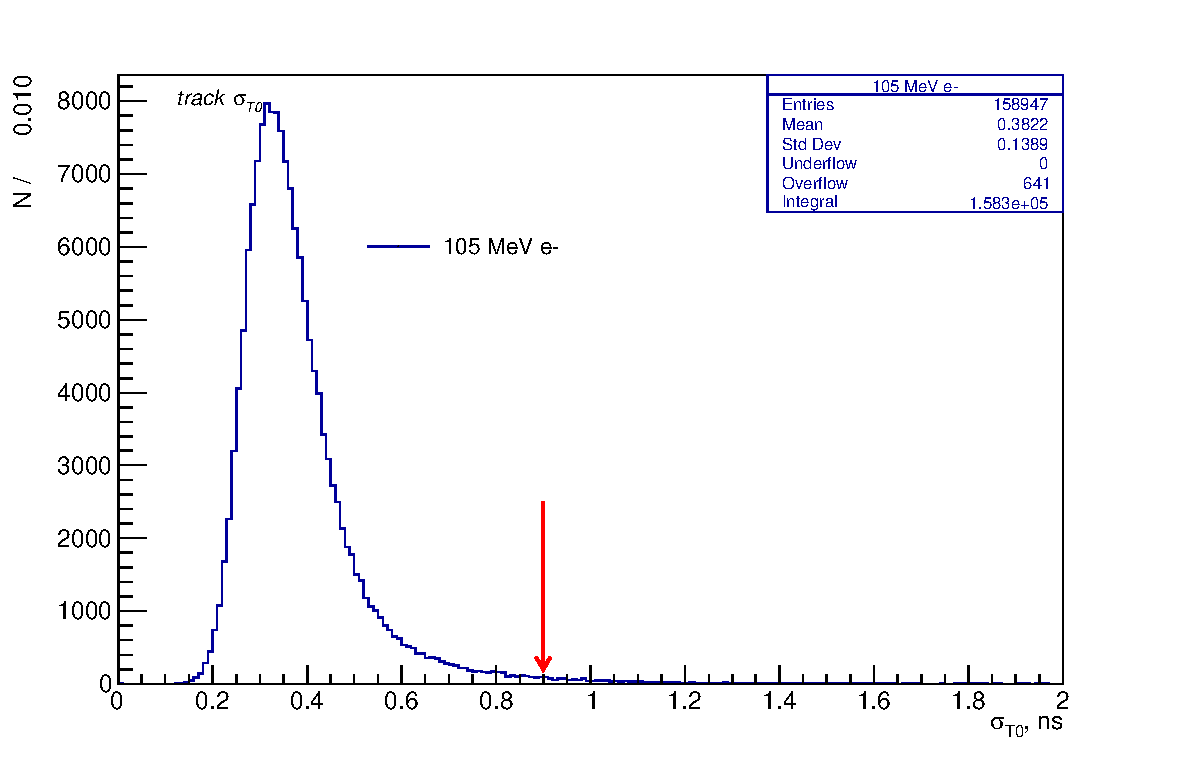
\includegraphics[width=0.60\textwidth]{figures/pdf/figure_00233_tid_1_t0err_1}
      % }
    };
    \node[anchor=south west,inner sep=0] at (11.,0.) {
      % \node[shift={(0 cm,0.cm)},inner sep=0,rotate={90}] at (0,0) {}
      % \makebox[\textwidth][c] {
      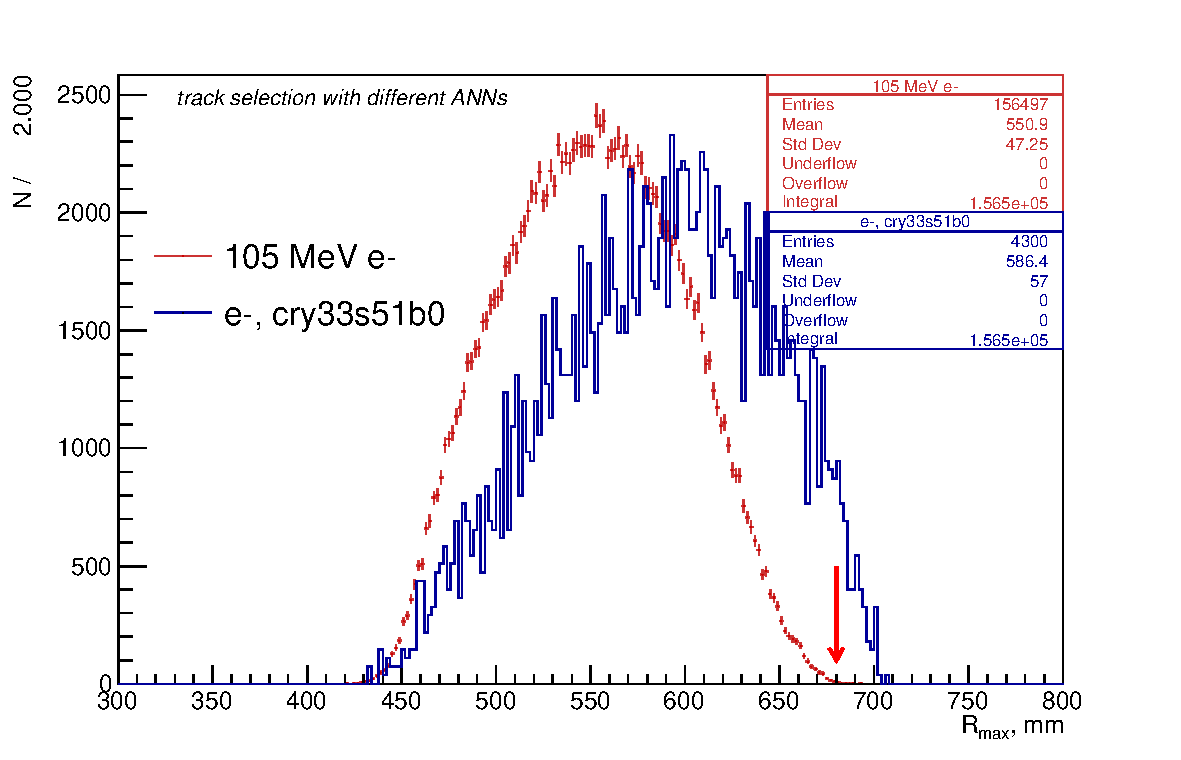
\includegraphics[width=0.60\textwidth]{figures/pdf/figure_00232_tid_1_rmax_1}
      % }
    };
    \node [text width=1cm, scale=0.8] at ( 2.5,5.4) {(a)};
    \node [text width=1cm, scale=0.8] at (13.5,5.4) {(b)};
  \end{tikzpicture}
  % \captionof{figure} {
  \caption{
    \label{fig:sigt0_1_and_rmax_1}
    (a): $\sigma_{T0}$ distribution for CE tracks; (b): $R_{max}$  distributions for CE (cele0s61b1) and cosmics (cry33s51b0).
    Tracks in the distributions pass all selections cuts except the cut on the plotted variable. Arrows shows the cut values.
  }
\end{figure}

Although the \MuToEm\ and \MuToEp\ analyses use different track quality ANN's trained using tracks
in a different momentum range, the cut value on the ANN score is the same in both cases.
It is confirmed that the ANN-based track selection is charge-symmetric, i.e. for a given momentum,
the track selection efficiency does not depend on the reconstructed track charge.
